\chapter{Preâmbulo matemático}
\textsl{{\sffamily(Versão: \today)}}

\section{Produto escalar e produto vetorial de vetores}
\subsection*{Produto escalar ou interno}
Dados dois vetores, define-se o seu \emph{produto escalar} (ou \emph{produto
interno}) como o escalar que se obtém multiplicando os módulos dos dois vetores
e o cosseno do ângulo entre eles. Assim, se $\vec a$ e $\vec b$ forem os dois
vetores e $\theta$ for o ângulo que definem, o produto escalar
é\footnote{Nestes apontamentos usa-se uma convenção tipográfica usual em física,
  em que se representa o módulo de um vetor $\vec a$ por $a$: a mesma letra, mas
sem a setinha por cima.}
\begin{equation}
  \vec a\cdot\vec b= ab\cos\theta.
\end{equation}
É imediato verificar que o produto escalar de dois vetores pode ser positivo (se
o ângulo entre eles for menor que 90\deg), negativo (se for maior que 90\deg) ou
nulo (se os dois vetores forem perpendiculares). Verifica-se também
que este produto é comutativo, isto é, $\vec a\cdot\vec b=\vec b\cdot\vec a$.

Sejam respetivamente $(a_x,\,a_y,\,a_z)$ e $(b_x,\,b_y,\,b_z)$ as componentes
dos vetores $\vec a$ e $\vec b$ relativamente a alguma base ortonormada
pré-escolhida, formada por versores (vetores com norma 1) $\he_x$, $\he_y$ e
$\he_z$. Isto quer dizer que estes dois vetores se podem escrever como as
combinações lineares dos vetores da base seguintes
\begin{align*}
  \vec a&=a_x\he_x+a_y\he_y+a_z\he_z&
  \vec b&=b_x\he_x+b_y\he_y+b_z\he_z.
\end{align*}
O produto escalar destes dois vetores pode então desenvolver-se como
\begin{align*}
  \vec a\cdot\vec b&=
  (a_x\he_x+a_y\he_y+a_z\he_z) \cdot (b_x\he_x+b_y\he_y+b_z\he_z)\\
  &=a_xb_x(\he_x\cdot\he_x)+ a_xb_y(\he_x\cdot\he_y)+ a_xb_z(\he_x\cdot\he_z)\\
  &+a_yb_x(\he_y\cdot\he_x)+ a_yb_y(\he_y\cdot\he_y)+ a_yb_z(\he_y\cdot\he_z)\\
  &+a_zb_x(\he_z\cdot\he_x)+ a_zb_y(\he_z\cdot\he_y)+ a_zb_z(\he_z\cdot\he_z)
\end{align*}
Mas os produtos escalares de versores da base diferentes são nulos (porque eles
são todos perpendicuares entre si) e os produtos escalares de um qualquer versor
da base consigo próprio é 1 (porque o módulo dos versores é 1 e o cosseno do
ângulo [nulo] que um vetor faz consigo próprio também é 1), isto é,
\begin{align*}
  \he_x\cdot\he_x=\he_y\cdot\he_y=\he_z\cdot\he_z=1\\
  \he_x\cdot\he_y=\he_y\cdot\he_z=\he_z\cdot\he_x=0.
\end{align*}
Substituindo em cima, obtemos uma forma alternativa para o produto escalar de
dois vetores:
\begin{equation}\label{eq:dprod}
  \vec a\cdot\vec b=a_xb_x+a_yb_y+a_zb_z.
\end{equation}

\subsection*{Produto vetorial ou externo}
Define-se também o \emph{produto vetorial} ou \emph{produto externo} de vetores.
Como o próprio nome indica, o produto vetorial de dois vetores é ainda um
vetor.
A norma do produto escalar de dois vetores é o produto
das suas normas e do seno do ângulo entre eles:
\begin{equation}
  \|\vec a\times\vec b\|=ab\sin\theta;
\end{equation}
a sua direção é a perpendicular ao plano definido pelos dois vetores que se
multiplicam e o sentido é o definido pela regra da mão direita\footnote{%
  \parbox[t]{0.8\textwidth}{Há várias formas de enunciar esta regra, pode
    encontrá-las todas rapidamente numa pesquisa na web (experimente usar
    ``cross product right hand rule'' como expressão de busca). Escolha a que
    preferir. Eu gosto desta: oriente o indicador da mão direita como o primeiro
    vetor no produto e o médio da mesma mão como o segundo; o polegar indica
  então o sentido do produto vetorial (veja a figura ao lado, retirada da
  Wikipedia)}\hfill
  \parbox[t]{1.8cm}{%
    \raisebox{-0.8\height}{%
      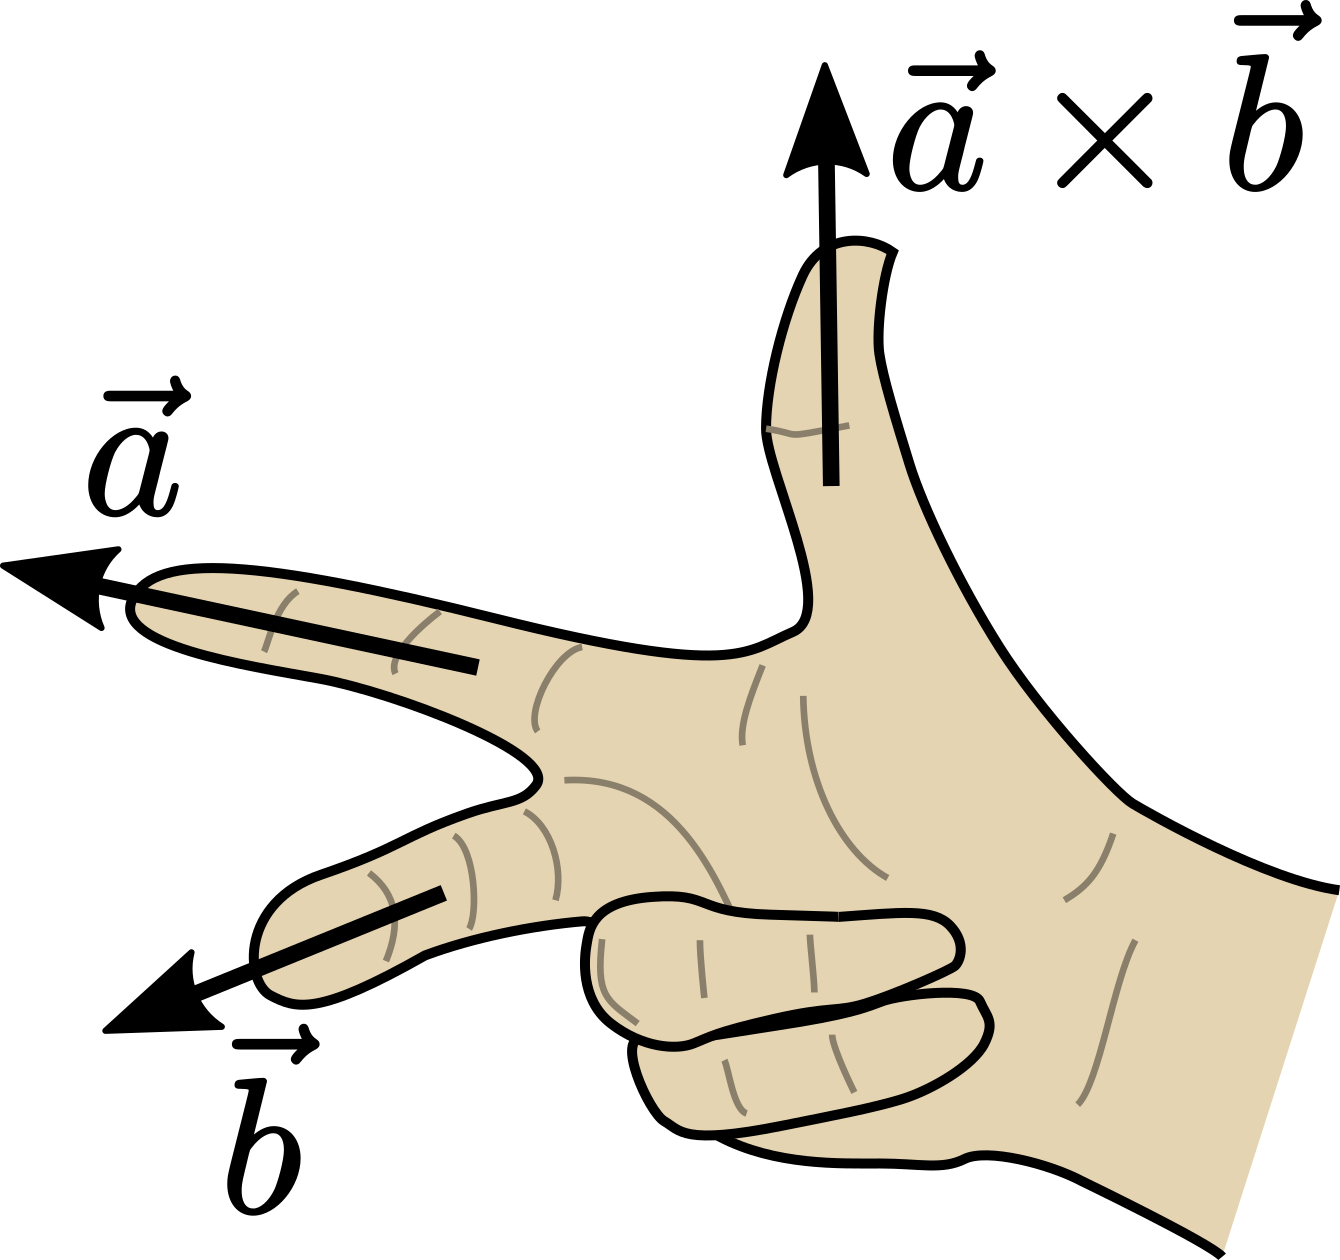
\includegraphics[width=1.7cm]{figs/f10-010.png}
    }
  }
}.
O produto vetorial assim definido é \emph{anticomutativo}, isto é, o sinal do
resultado é trocado se trocarmos a ordem dos fatores: $\vec a\times\vec b=-\vec
b\times\vec a$. Constata-se também que
\begin{align}
  \he_x\times\he_y&=\he_z&
  \he_y\times\he_z&=\he_x&
  \he_z\times\he_x&=\he_y.
\end{align}
Munidos destas igualdades (e das que resultam trocando a ordem dos fatores nos
seus lados esquerdos) obtemos uma expressão para o cálculo do vetor produto
vetorial em termos das componentes dos dois vetores multipicados externamente.
Sejam, como há pouco, $a_x,\,a_y,\,a_z$ e $b_x,\,b_y,\,b_z$ as componentes de
dois vetores $\vec a $ e $\vec b$ relativamente a uma base ortonormada formada
por vetores unitarios $\he_x$ $\he_y$, $\he_z$. Então,
\begin{equation*}
  \vec a = a_x\he_x+a_y\he_y+a_z\he_z\rule{2cm}{0mm}
  \vec b = b_x\he_x+b_y\he_y+b_z\he_z,
\end{equation*}
e, assim,
\begin{align*}
  \vec a \times \vec b &=
  (a_x\he_x+a_y\he_y+a_z\he_z)\times
  (b_x\he_x+b_y\he_y+b_z\he_z)\\
  &=
  (a_yb_z-a_zb_y)\he_x+(a_zb_x-a_xb_z)\he_y+(a_xb_y-a_yb_x)\he_z.
\end{align*}
Esta expressão para o produto vetorial de dois vetores em termos das componentes
dos vetores multiplicados é fácil de memorizar notando que pode também ser vista
como o determinante da matriz simbólica (verifique):
\begin{equation}
  \vec a\times\vec b =\det
  \begin{bmatrix}
    \he_x&\he_y&\he_z\\
    a_x&a_y&a_z\\
    b_x&b_y&b_z
  \end{bmatrix}.
\end{equation}

O produto vetorial não é comutativo (é anticomutativo, como vimos) e também não
é associativo. O produto vetorial de três vetores satisfaz as igualdades
\begin{equation}\label{eq:tcp}
\begin{split}
\vec a\times(\vec b\times\vec c)&=\vec b(\vec a\cdot\vec c)-(\vec a\cdot\vec
b)\vec c\\
(\vec a\times\vec b)\times\vec c&=\vec b(\vec a\cdot\vec c)-\vec a(\vec
b\cdot\vec c)
\end{split}
\end{equation}

\subsection*{Áreas de paralelogramos e volumes de paralelipípedos}
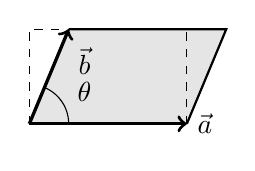
\begin{tikzpicture}[baseline=(current bounding box.north)]
%\small
\coordinate(O) at (0,0);
\coordinate(a) at (2,0);
\coordinate(b) at (0.5,1.2);
\coordinate(ab) at (2.5,1.2);
\fill [gray!20] (O) -- (a) -- (ab) -- (b) --cycle;
\draw [very thick, ->] (O) --(a) node[right]{$\vec a$};
\draw [very thick, ->] (O) --(b) node[shift={(2mm,-4mm)}]{$\vec b$};
\draw [thick] (a) -- (ab) -- (b);
\draw [dashed] (O) -- (O|-b) --(b);
\draw [dashed] (a) -- (a|-b);
\begin{scope}
\clip (b)--(O) --(a);
\draw (O) circle (0.5cm) node[shift={(7mm,4mm)}] {$\theta$};
\end{scope}
\end{tikzpicture}
\hfill
\begin{minipage}[t]{0.8\textwidth}
Consideremos a área do paralelogramo formado por dois vetores $\vec a$ e $\vec
b$ (ver a figura ao lado). Seja $\theta$ o ângulo entre os dois vetores.
Claramente, aquela área é igual à do retângulo com base $a=\|\vec a\|$ e altura
$b\sin\theta$, igual à do paralelogramo inicial. A área considerada é pois
\end{minipage}
\begin{equation}
A=ab\sin\theta=\|\vec a\times\vec b\|.
\end{equation}

Consideremos agora um terceiro vetor $\vec c$, não coplanar com $\vec a$ e $\vec
b$. Seja $\phi$ o ângulo entre $\vec c$ e a normal ao plano definido pelos
vetores $\vec a$ e $\vec b$. Com um argumento semelhante ao que acabámos de
usar para calcular a área de um paralelogramo, prova-se que o volume deste
paralelipípedo é
\begin{equation}
V=b\cos\phi A = c \|\vec a\times\vec b\| \cos\phi=
\left|\vec c\cdot\vec a\times\vec b\right|.
\end{equation}

\section{Sistemas de coordenadas e bases de vetores}
Um sistema de coordenadas é uma forma de especificar numericamente a posição de
cada ponto no espaço. Porque o espaço em que nos movemos é tridimensional, são
em geral necessários três números (três coordenadas) para definir completamente
a posição de cada ponto. Em certas situações, a posição dos objetos considerados
pode estar constrangida de algum modo e, por isso, bastarem dois (como a
latitude e a longitude de um ponto na superfície da Terra) ou apenas um (o
\emph{quilómetro} onde se dá um acidente numa autoestrada) para a especificar;
nestes casos, o espaço considerado é apenas bi- ou unidimensional.

O sistema de coordenadas usado em cada problema é definido como for considerado
mais conveniente. Qualquer problema pode ser analisado com qualquer sistema de
coordenadas, mas a complexidade algébrica da análise pode ser muito diferente
usando diferentes sistemas.

Os sistemas mais frequentemente usados em física (mas de modo algum os únicos)
são os seguintes (veja a Figura~\ref{fig:10-015}):
\begin{itemize}
\item\textbf{coordenadas cartesianas $(x,\,y,\,z)$}\\
    O sistema de coordenadas mais familiar é o das coordenadas cartesianas.
    Escolhido um ponto (a origem) e três direções perpendiculares entre si (os
    \emph{eixos coordenados} das coordenadas $x$, $y$ e $z$, indicamos a posição
    de um ponto dado pelas distâncias que o separam de cada um dos planos
    definidos por cada par de eixos coordenados, eventualmente afetadas de um
    sinal para indicar de que lado de cada plano se encontra o ponto.
\item\textbf{coordenadas polares esféricas $(r,\,\theta,\,\phi)$}\\
    Outro sistema muito usual é o das coordenadas polares esféricas. Escolhida a
    origem, uma direção que a contém (o eixo \emph{polar}) e um plano que contem
    o eixo (plano de referência azimutal), a posição de um ponto é indicada pela
    sua distância à origem $r$, pelo ângulo $\theta$ (chamado \emph{ângulo
    polar}) que a linha que o une à origem faz com o eixo polar e pelo ângulo
    $\phi$ (\emph{ângulo azimutal}) que essa linha faz com o plano de referência
    azimutal.
\item\textbf{coordenadas polares cilíndricas $(\rho,\,z,\,\phi)$}\\
    De certa maneira, o sistema de coordenadas polares cilíndricas é um misto
    das coordenadas cartesianas e das coordenadas polares esféricas. Com nas
    coordenadas esféricas, escolhe-se uma origem, um eixo polar e um plano de
    referência azimutal; a partir daí, usa-se a distância $\rho$ do ponto ao
    eixo polar (atenção: é a distância ao eixo, não a distância à origem), a
    distância $z$ do ponto ao plano perpendicular a esse eixo que contém a
    origem (corresponde à coordenada cartesiana $z$ se tomarmos o eixo polar
    como eixo dos $z$) e o ângulo azimutal $\phi$ para especificar a sua
    posição.
\end{itemize}
\begin{figure}[htb]
{\centering
\tdplotsetmaincoords{65}{120}
%
\pgfmathsetmacro{\rvec}{0.9}
\pgfmathsetmacro{\thetavec}{30}
\pgfmathsetmacro{\phivec}{50}
%
\begin{tikzpicture}[scale=3,tdplot_main_coords]
    % Cartesian
    \begin{scope}[xshift=-1.5cm]
        \coordinate (O) at (0,0,0);
        \draw[->] (O) -- (0.5,0,0);  %x
        \draw[->] (O) -- (0,0.5,0);  %y
        \draw[->] (O) -- (0,0,0.88); %z

        \tdplotsetcoord{P}{\rvec}{\thetavec}{\phivec}
        \draw[-stealth] (O) -- (P) node[above right] {$P$};
        \draw [thin, dashed] (O) -- (Pxy);
        \draw [thin, dashed] (P) -- (Pxy);
        \draw [thin, dashed] (P) -- (Pz) node[left]{$z$};
        \draw [thin, dashed] (Px) node [above] {$x$} --(Pxy)--(Py) node[above]
        {$y$};
    \end{scope}
    % Polar Spherical
    \begin{scope}
        \coordinate (O) at (0,0,0);
        \draw[->] (O) -- (0.5,0,0);  %x
        \draw[->] (O) -- (0,0.5,0);  %y
        \draw[->] (O) -- (0,0,0.88); %z

        \tdplotsetcoord{P}{\rvec}{\thetavec}{\phivec}
        \draw[-stealth] (O) -- (P) node[above right] {$P$}
            node [pos=0.7, shift={(0.0,0.05,-0.25)}] {$r$};
        \draw [thin, dashed] (O) -- (Pxy);
        \draw [thin, dashed] (P) -- (Pxy);
        \draw [thin, dashed] (P) -- (Pz);
        %\draw [thin, dashed] (Px) --(Pxy)--(Py);

        \tdplotdrawarc[thin]{(O)}{0.25}{0}{\phivec}{anchor=north}{$\phi$}
        \tdplotsetthetaplanecoords{\phivec}
        \tdplotdrawarc[tdplot_rotated_coords,thin]{(0,0,0)}{0.4}{0}%
            {\thetavec}{anchor=south,xshift=1.5}{$\theta$}
    \end{scope}
    % Polar Cilyndrical
    \begin{scope}[xshift=1.5cm]
        \coordinate (O) at (0,0,0);
        \draw[->] (O) -- (0.5,0,0);  %x
        \draw[->] (O) -- (0,0.5,0);  %y
        \draw[->] (O) -- (0,0,0.88); %z

        \tdplotsetcoord{P}{\rvec}{\thetavec}{\phivec}
        \draw[-stealth] (O) -- (P) node[above right] {$P$};
        \draw [thin, dashed] (O) -- (Pxy);
        \draw [thin, dashed] (P) -- (Pxy);
        \draw [thin, dashed] (P) -- (Pz) node[left]{$z$} node
        [midway,shift={(2pt,5pt)}]{$\rho$};
       % \draw [thin, dashed] (Px) --(Pxy)--(Py);

        \tdplotdrawarc[thin]{(O)}{0.25}{0}{\phivec}{anchor=north}{$\phi$}
        \tdplotsetthetaplanecoords{\phivec}
    \end{scope}
\end{tikzpicture}\par
}
\caption{Coordenadas cartesianas $(x,\,y,\,z)$ (à esquerda), coordenadas polares
esféricas $(r,\,\theta,\,\phi)$ (ao centro) e coordenadas polares cilíndricas
$(\rho,\,z,\,\phi)$ (à direita).\label{fig:10-015}}
\end{figure}

Escolhendo para eixo polar o eixo da coordenada cartesiana $z$ e o plano de
referência azimutal coincidente com o plano $zx$, as relações entre as coordenadas
cartesianas e as coordenadas polares esféricas (colunas da esquerda) e
cilíndricas (colunas da direita) são
\begin{align}
x&=r\sin\theta\cos\phi&
    r&=\sqrt{x^2+y^2+z^2}\hspace{2.0cm}&
    x&=\rho\cos\phi&
    \rho&=\sqrt{x^2+y2}\nonumber\\
y&=r\sin\theta\sin\phi&
    \theta&=\arccos\frac{z}{r}&
    y&=\rho\sin\phi&
    \phi&=\arctan\frac{y}{x}\label{eq:polarcoords}
    \\
    z&=r\cos\theta&
    \phi&=\arctan\frac{y}{x}&
    z&=z&\nonumber
\end{align}

Quando lidamos com variáveis vetoriais, é conveniente dispormos de \emph{bases}
de vetores, que usamos para as descrever. Por exemplo, a aceleração da
gravidade é uma variável vetorial que, perto da superfície da Terra, tem direção
vertical, dirigida para baixo e o seu módulo tem o valor 9,8\,m/s$^2$.
Escolhendo uma base formada por dois versores (vetores com norma unitária)
horizontais $\he_x$ e $\he_y$ e um terceiro vetor $\he_z$ vertical, orientado
para cima, podemos resumir esta descrição na expressão $\smash{\vec
g=-9,8\,\text{m/s}^2}\,\he_z$ ou $\smash{\vec g=(0,\,0,\,-9,8\,\text{m/s}^2)}$,
usando outra notação habitual.  Qualquer destas notações só fica definida depois
de estar escolhida a base usada. 

Este problema da escolha da base é independente do da escolha do sistema de
coordenadas. Ainda assim, é usual escolherem-se os vetores que formam a base
vetorial paralelos, em cada ponto, aos eixos coordenados\footnote{Isto é, às
direções em que apenas uma das coordenadas varia.} nesse ponto, caso em
que chamamos à base assim definida base do sistema de coordenadas usado.
Assim, concretizando para o sistema de coordenadas cartesiano, mais familiar,
escolhemos o versor $\he_x$ da base das coordenadas cartesianas orientado na
direção em que a coordenada $x$ aumenta, ficando as restantes ($y$ e $z$)
constantes, e repetindo a lógica para os restantes vetores $\he_y$ e $\he_z$. Do
mesmo modo, o versor $\he_r$ da base das coordenadas esféricas tem, em cada
ponto, a direção em que a coordenada $r$ aumenta sem variarem as coordenadas
$\theta$ ou $\phi$. Tem pois a direção radial. A Figura~\ref{fig:10-016} ilustra
as orientações dos vetores das bases dos três sistemas de coordenadas referidos.
\begin{figure}[htb]
{\centering
\tdplotsetmaincoords{65}{120}
%
\pgfmathsetmacro{\rvec}{0.9}
\pgfmathsetmacro{\thetavec}{30}
\pgfmathsetmacro{\phivec}{50}
%
\begin{tikzpicture}[scale=3,tdplot_main_coords]
    % Cartesian
    \begin{scope}[xshift=-1.5cm]
        \coordinate (O) at (0,0,0);
        \draw[->] (O) -- (0.5,0,0);  %x
        \draw[->] (O) -- (0,0.5,0);  %y
        \draw[->] (O) -- (0,0,0.88); %z

        \tdplotsetcoord{P}{\rvec}{\thetavec}{\phivec}
        \draw[-stealth] (O) -- (P);
        \draw [thin, dashed] (O) -- (Pxy);
        \draw [thin, dashed] (P) -- (Pxy);
        \draw [thin, dashed] (P) -- (Pz) node[left]{$z$};
        \draw [thin, dashed] (Px) node [above] {$x$} --(Pxy)--(Py) node[above]
        {$y$};
        \draw [thick,->] (P) -- +(0,0,0.2) node[above]{$\hat e_z$};
        \draw [thick,->] (P) -- +(0,0.2,0) node[right]{$\hat e_y$};
        \draw [thick,->] (P) -- +(0.28,0,0) node[left]{$\hat e_x$};
    \end{scope}
    % Polar Spherical
    \begin{scope}
        \coordinate (O) at (0,0,0);
        \draw[->] (O) -- (0.5,0,0);  %x
        \draw[->] (O) -- (0,0.5,0);  %y
        \draw[->] (O) -- (0,0,0.88); %z

        \tdplotsetcoord{P}{\rvec}{\thetavec}{\phivec}
        \draw[-stealth] (O) -- (P)
            node [pos=0.7, shift={(0.0,0.05,-0.25)}] {$r$};
        \draw [thin, dashed] (O) -- (Pxy);
        \draw [thin, dashed] (P) -- (Pxy);
        \draw [thin, dashed] (P) -- (Pz);
        %\draw [thin, dashed] (Px) --(Pxy)--(Py);

        \tdplotdrawarc[thin]{(O)}{0.25}{0}{\phivec}{anchor=north}{$\phi$}
        \tdplotsetthetaplanecoords{\phivec}
        \tdplotdrawarc[tdplot_rotated_coords,thin]{(0,0,0)}{0.4}{0}%
            {\thetavec}{anchor=south,xshift=1.5}{$\theta$}
        \tdplotsetrotatedcoords{\phivec}{\thetavec}{0}
        \tdplotsetrotatedcoordsorigin{(P)}
        \draw[thick,tdplot_rotated_coords,->] (0,0,0)
            -- (.15,0,0) node[right]{$\hat e_\theta$};
        \draw [thick,tdplot_rotated_coords,->] (0,0,0) -- (0,0.14,0)
            node[right]{$\hat e_\phi$};
        \draw [thick,tdplot_rotated_coords,->] (0,0,0) -- (0,0,0.25)
            node[above]{$\hat e_r$};
    \end{scope}
    % Polar Cilyndrical
    \begin{scope}[xshift=1.5cm]
        \coordinate (O) at (0,0,0);
        \draw[->] (O) -- (0.5,0,0);  %x
        \draw[->] (O) -- (0,0.5,0);  %y
        \draw[->] (O) -- (0,0,0.88); %z

        \tdplotsetcoord{P}{\rvec}{\thetavec}{\phivec}
        \draw[-stealth] (O) -- (P);
        \draw [thin, dashed] (O) -- (Pxy);
        \draw [thin, dashed] (P) -- (Pxy);
        \draw [thin, dashed] (P) -- (Pz) node[left]{$z$} node
            [midway,shift={(-1pt,-6pt)}]{$\rho$};

        \draw [thick,->] (P) --+(0,0,0.17) node[above]{$\hat e_z$};
        \draw [thick,->] (P) -- ($ (P)!-0.15cm!(Pz) $) node [right]{$\hat
        e_\rho$};
        \tdplotdrawarc[thin]{(O)}{0.25}{0}{\phivec}{anchor=north}{$\phi$}
        \tdplotsetthetaplanecoords{\phivec}

        \tdplotsetrotatedcoords{\phivec}{\thetavec}{0}
        \tdplotsetrotatedcoordsorigin{(P)}
        \draw [thick,tdplot_rotated_coords,->] (0,0,0) -- (0,0.14,0)
            node[right]{$\hat e_\phi$};
    \end{scope}
\end{tikzpicture}\par
}
\caption{Bases dos três sistemas de coordenadas mais usuais: cartesiano
(esquerda), polar esférico (centro), polar
cilíndrico(direita).\label{fig:10-016}}
\end{figure}
Note-se que as orientações dos vetores da base de um sistema de coordenadas não
são, em geral, constantes. Antes pelo contrário, elas são, normalmente, funções da
posição. Por exemplo, a orientação do vetor $\he_r$ da base das coordenadas
polares é, como já se disse, radial. A direção radial é a da linha que une a
origem ao ponto considerado; logo, depende de ponto para ponto. A principal
excepção a esta regra geral é a dos vetores da base das coordenadas cartesianas:
$\he_x$, $\he_y$ e $\he_z$ mantêm as suas orientações inalteradas em todos os
pontos do espaço.

\subsection*{Porque usar coordenadas não cartesianas}
Já disse que o sistema de coordenadas a usar é escolhido como se julgar mais
conveniente. Qualquer problema resolúvel usando um sistema de coordenadas pode
ser resolvido usando outro qualquer. Mas as propriedades de simetria do problema
podem, escolhendo apropriadamente o sistema de coordenadas, ser exploradas para
simplificar a sua formulação e resolução. Vejamos alguns exemplos.
\begin{examples}
\item A forma de uma superfície esférica com raio $a$ e centro na origem, em
  coordenadas cartesianas e em coordenadas esféricas.\\
  Os pontos da superfície esférica estão todos à mesma distância do centro, ou
  seja, da origem do sistema de coordenadas. Assim, em coordenadas esféricas
  dizemos que a superfície é formada pelos pontos do conjunto
  \begin{equation*}
    S=\{(r,\theta,\phi): r=a\};
  \end{equation*}
  em coordenadas cartesianas, a distância à origem é dada por
  $r=\sqrt{x^2+y^2+z^2}$, de forma que o conjunto dos pontos que formam a
  superfície é agora definido como
  \begin{equation*}
    S=\{(x,y,z): \sqrt{x^2+y^2+z^2}=a\}.
  \end{equation*}
  A descrição em coordenadas esféricas é muito mais simples.
\item
  Potencial gravitacional do Sol.\\
  O potencial gravitacional do Sol é, nos pontos exteriores ao próprio Sol,
  proporcional à massa solar e inversamente proporcional à distância ao seu
  centro. Em coordenadas esféricas $(r,\,\theta,\,\phi)$ com origem no centro do
  Sol, a expressão matemática desta função é
  \begin{equation*}
    V(r,\theta,\phi)=-G\frac{M}{r},
  \end{equation*}
  onde $G$ é uma constante universal (constante da gravitação universal) e $M$ a
  massa solar.\\
  Em coordenadas cartesianas ($x,\,y,\,z)$ com origem também no centro do Sol, a
  mesma função da posição assume a forma
  \begin{equation*}
    V(x,y,z)=-G\frac{M}{\sqrt{x^2+y^2+z^2}}.
  \end{equation*}
  Claramente, o potencial gravitacional solar (ou de outro corpo qulquer com
  forma esférica) tem uma expressão mais simples em coordenadas esféricas do que
  em coordenadas cartesianas, porque a própiar função tem simetria esférica.
\item
  Campo elétrico gerado por um fio retilíneo infinitamente comprido,
  uniformemente carregado.\\
  Um fio retilíneo de comprimento infinito, uniformemente carregado, gera, nos
  pontos à sua volta, um campo elétrico com direção radial (isto é, em cada
  ponto perpendicular à direção do fio, distribuído em torno do fio como os
  raios de uma roda de bicicleta se distribuem em torno do seu eixo), com uma
  intensidade inversamente proporcional à distância ao fio. Em coordenadas
  polares cilíndricas $(\rho,z,\phi)$ com eixo polar coincidente com o fio
  carregado, a expressão do campo é
  \begin{equation*}
    \vec E(\rho,z,\phi)=\frac{1}{2\pi\epsilon_0}\frac{\lambda}{\rho}\he_\rho,
  \end{equation*}
  onde $\lambda$ é a densidade linear de carga e $\epsilon_0$ é uma constante
  universal (permitividade elétrica do vacuo).
  Em coordenadas cartesianas com o eixo dos $zz$ coincidente com o fio
  carregado, temos
  \begin{equation*}
    \vec E(x,y,z)=\frac{\lambda}{2\pi\epsilon_0}\frac{x\he_x+y\he_y}{x^2+y^2}.
  \end{equation*}
  Mais uma vez, as coordenadas cartesianas não permitem a descrição mais simples
  simples possível.
\end{examples}

\section{Representações gráficas de funções da posição}
As representações gráficas de funções da posição numa superfície ou no espaço
são complicadas porque há sempre mais variáveis envolvidas do que dimensões no
plano onde se desenha a representação. No caso de funções escalares definidas
numa superfície (por exemplo, a temperatura superficial numa chapa de vidro, a
espessura da película de água que delimita uma bola de sabão, ou a altitude numa
região geográfica), a opção mais usual é a de usar um \emph{mapa de cores,} onde
se faz corresponder diferentes cores a diferentes valores da função; outra
possibilidade é a da representação por \emph{contornos} ou \emph{linhas de
nível,} onde se desenham linhas que unem pontos onde a função tem valor (nível)
constante. A Figura~\ref{fig:plot2d} ilustra estas duas possibilidades.
\begin{figure}[htb]
{\centering
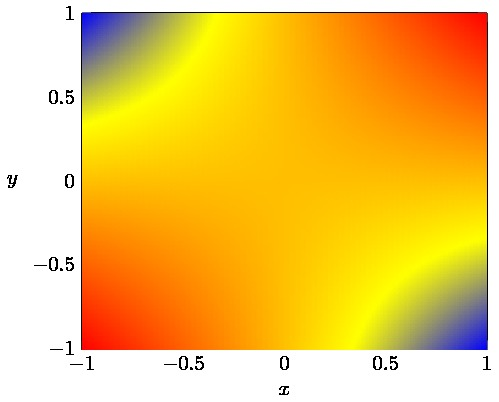
\includegraphics[width=0.4\linewidth]{figs/f10-plot2d-surf}\hspace{5mm}
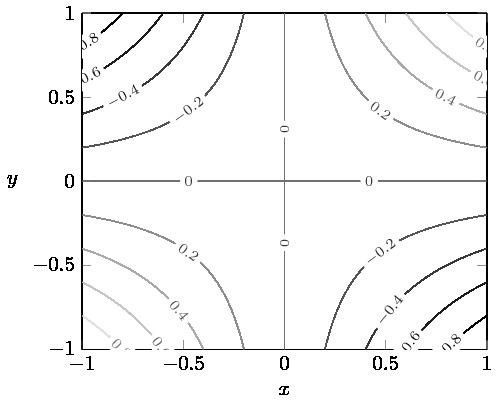
\includegraphics[width=0.4\linewidth]{figs/f10-plot2d-cont}\hspace{5mm}
\par
}
\caption{Duas representações gráficas da função $f(x,y)=xy$. À esquerda, por
mapa de cores; à direita por linhas de nível.\label{fig:plot2d}}
\end{figure}

Em três dimensões, as linhas de nível são antes \emph{superfícies de nível} e a
representação gráfica torna-se ainda mais complicada, mas é ainda possível. Por
exemplo, são usuais as representações das superfícies de nível da função
probabilidade de presença eletrónica nas orbitais atómicas dos átomos
hidrogenóides (Figura~\ref{fig:orbitals})
\begin{figure}[htb]
{\centering
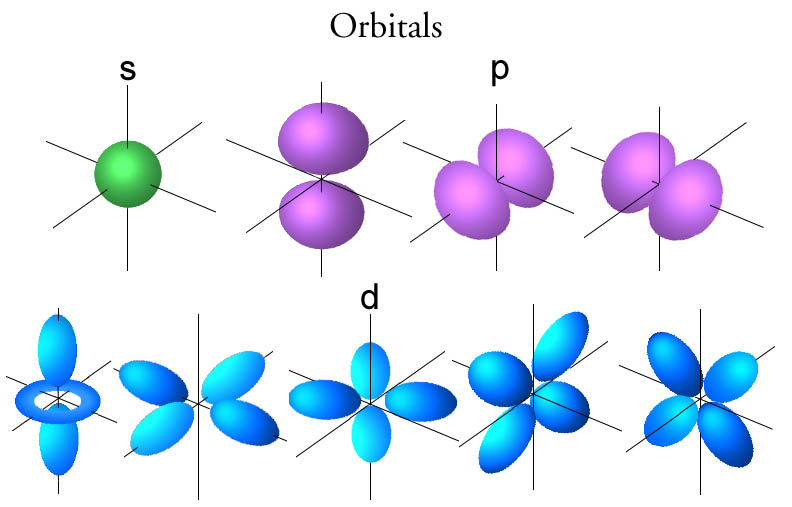
\includegraphics[width=0.5\linewidth]{figs/f10-030.jpg}
\par
}
\caption{Representação gráfica de algumas orbitais eletrónicas do átomo de
hidrogénio. As superfícies desenhadas são superfícies de nível da função (da
posição) densidade de probabilidade de presença do eletrão. (Imagem retirada de
\protect\url{http://chemsite.lsrhs.net/bonding/configs.html})%
\label{fig:orbitals}}
\end{figure}

A representação gráfica de funções vetoriais (por exemplo, o campo da velocidade
do escoamento da água num rio, ou o campo elétrico gerado por uma distribuição
de cargas) é ainda mais difícil porque para além da intensidade da função, deve
ainda dar-se informação sobre a sua orientação. Uma possibilidade comum é fazer
uma mapa de setas, onde se desenha uma malha de setinhas que representam a
função em cada ponto. Mas a opção mais útil e clara é a representação por
\emph{linhas de força,} linhas que são em cada ponto tangentes à direção da
função. Nesta representação não é dada uma ideia direta da intensidade da função,
apenas da sua orientação. Porém, para todas as funções com interesse físico,
verifica-se que têm maior intensidade nas regiões onde as linhas de força se
encontram mais próximas umas das outras.  A Figura~\ref{fig:dipole} ilustra as
linhas de força do campo elétrico gerado por duas cargas de sinal oposto mas
igual módulo.
\begin{figure}[htb]
{\centering
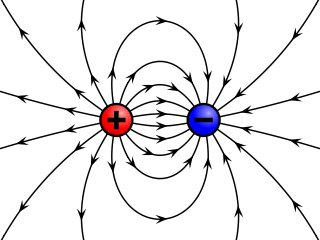
\includegraphics[width=0.4\textwidth]{figs/f10-dipole.png}
\par
}
\caption{representação por linhas de força do campo elétrico gerado por duas
cargas de igual módulo e sinal oposto. (Imagem retirada de 
\protect\url{https://commons.wikimedia.org/wiki/File:VFPt_dipole_electric.svg}.)
\label{fig:dipole}}
\end{figure}



\section{Funções de várias variáveis e derivadas parciais}
Seja $f(v_1,\,v_2,\,\ldots,v_N)$ uma função contínua de $N$ variáveis $v_1$,
$v_2$, \ldots, $v_N$. Por \emph{função} entendemos apenas uma aplicação
puramente matemática sem qualquer significado físico, uma regra de cálculo
para a determinação de um \emph{resultado} (o \emph{valor} da função) a partir
dos valores das variáveis $v_1$, $v_2$, \ldots, $v_N$. Por exemplo, 
$f(a,\,b)=2a+\exp(a-b)$ é uma função contínua das variáveis $a$ e $b$. Dizemos
que uma função é contínua no sentido em que se as variáveis $v_k$ sofrerem
\emph{pequenas} variações, a função irá também variar apenas
\emph{ligeiramente}\footnote{Esta noção de continuidade é absurdamente
imprecisa, mas o seu significado intuitivo é aqui suficiente.}.

Tratando-se de uma função contínua, a sua variação, 
\begin{equation*}
\delta f=f(v_1+\delta v_1,\,v_2+\delta v_2,\,\ldots,\,v_N+\delta v_N)-
f(v_1,\,v_2,\,\ldots,\,v_N),
\end{equation*}
quando as variáveis de que depende sofrem variações $\delta v_1$, $\delta v_2$,
\ldots, $\delta v_N$ deve ser, em primeira ordem de aproximação, uma combinação
linear das variações das variáveis,
\begin{equation}\label{eq:dfp}
\delta f\simeq A_1\delta v_1+A_2\delta v_2+\ldots+A_N\delta v_N,
\end{equation}
onde os coeficientes $A_k=A_k(v_1,\,\ldots,\,v_N)$ são funções das variáveis
$v_1$, $v_2$, etc., mas não dos seus acréscimos $\delta v_1$, $\delta v_2$, etc.
Consideremos uma situação em que todos os acréscimos excepto o da primeira
variável $v_1$ se anulam, isto é,
\begin{align*}
\delta v_1&\neq0&\delta v_2&=\delta v_3=\ldots=\delta v_N=0.
\end{align*}
A igualdade aproximada da eq.~\eqref{eq:dfp} reduz-se então a 
\begin{equation*}
\delta f\simeq f(v_1+\delta v_1,\,v_2,\,\ldots,\,v_N)-
    f(v_1,\,v_2,\,\ldots,\,v_N)= A_1\delta v_1,
\end{equation*}
de onde se obtem uma expressão aproximada para o coeficiente $A_1$:
\begin{equation*}
A_1\simeq
    \frac{f(v_1+\delta v_1,\,v_2,\,\ldots,\,v_N)
              -f(v_1,\,v_2,\,\ldots,\,v_N)}{\delta v_1}.
\end{equation*}
No limite $\delta v_1\rightarrow0$, o erro da aproximação deve anular-se, e o
coeficiente $A_1$ fica dado por
\begin{equation*}
A_1=\lim_{\delta v_1\rightarrow0}
    \frac{f(v_1+\delta v_1,\,v_2,\,\ldots,\,v_N)
              -f(v_1,\,v_2,\,\ldots,\,v_N)}{\delta v_1}.
\end{equation*}
O objeto assim definido é uma taxa de variação da função, ou seja, é uma
derivada da função $f$, chamada \emph{derivada parcial de $f$ em ordem a $v_1$}
e é normalmente representada com a notação $\partial f/\partial v_1$. De modo
semelhante definimos as restantes derivadas parciais da função $f$:
\begin{equation}
    \pd{f}{v_k} = \lim_{\delta v_k\rightarrow0}
    \frac{f(v_1,\,\ldots,\,v_k+\delta v_k,\,\ldots,\,v_N)-
        f(v_1,\,\ldots,\,v_N)}{\delta v_k},\qquad k=1,\,\ldots,\,N.
\end{equation}
Usando estas definições podemos dar uma forma mais informativa à
eq.~\eqref{eq:dfp}:
\begin{equation}\label{eq:df}
\delta f(v_1,\,v_2,\,\ldots,\,v_N)=\pd{f}{v_1}\delta v_1+\pd{f}{v_2}\delta v_2
    +\ldots+ \pd{f}{v_N}\delta v_N.
\end{equation}

Na prática, o cálculo das derivadas parciais de uma função de várias variáveis é
tão simples como o do cálculo da derivada de uma função de uma só variável.
Quando calculamos a derivada parcial em ordem a uma das variáveis de que depende
a função, tomamos todas as restantes variáveis como se fossem constantes. Assim,
por exemplo, dada a função $f(x,y)=xy$, temos
\begin{align*}
f(x,y)&=xy&\pd{f}{x}&=y,&\pd{f}{y}=x.
\end{align*}

\begin{examples}
\item Calcule as derivadas parciais da fução distância à origem
$r=\sqrt{x^2+y^2+z^2}$ relativamente às coordenadas cartesianas $x$, $y$ e $z$.
\\
Por exemplo, 
\begin{align*}
\pd{r}{x}&=\pd{}{x}\left(x^2+y^2+z^2\right)^{1/2}=
    \frac{1}{2}\left(x^2+y^2+z^2\right)^{-1/2}\;\pd{x^2}{x}
=\frac{x}{\sqrt{x^2+y^2+z^2}}=\frac{x}{r}.
\end{align*}
de igual modo se verifica que
\begin{align*}
\pd{r}{y}&=\frac{y}{r}& \pd{r}{z}&=\frac{z}{r}
\end{align*}
\end{examples}

\section{Vetor deslocamento em coordenadas não cartesianas}
Consideremos um ponto do espaço que se desloca.  Nesse deslocamento, as
coordenadas da sua posição vão variando, naturalmente. Usando coordenadas
cartesianas e a respetiva base, a expressão da variação do vetor posição como
função das variações das coordenadas é particularmente simples:
\begin{equation*}
  \delta \vec r= \delta x\he_x+\delta y\he_y+\delta z\he_z.
\end{equation*}
Vejamos agora como exprimir esta variação do vetor posição usando sistemas de
coordenadas arbitrários. Antes, porém, vamos introduzir a notação alternativa
seguinte para as coordenadas cartesianas:
\begin{align*}
  x_1&=x&\he_1&=\he_x\\
  x_2&=y&\he_2&=\he_y\\
  x_3&=z&\he_3&=\he_z.
\end{align*}
Esta notação permite escrever muitas expressões de forma mais compacta. Por
exemplo,
\begin{equation}\label{eq:drcart}
  \delta\vec r= \delta x\he_x+\delta y\he_y+\delta z\he_z
  =x_1\he_1+ x_2\he_2+ x_3\he_3=\sum_{i=1}^3x_i\he_i.
\end{equation}

Introduzindo-se um outro sistema de coordenadas $(v_1, v_2, v_3)$, podemos
escrever, usando a regra da derivação da fução composta,
\begin{equation*}
\delta x_i=\sum_{j=1}^3\delta v_j\pd{x_i}{v_j},
\end{equation*}
de forma que
\begin{equation}\label{eq:drmixcoords}
  \delta\vec r=\sum_{i=1}^3\delta x_i\he_i=\sum_{i=1}^3\sum_{j=1}^3\delta v_j
  \pd{x_i}{v_j}\he_i=\sum_{j=1}^3\delta v_j\vec w_j,
\end{equation}
onde se introduziram os vetores
\begin{equation*}
  \vec w_j=\sum_{i=1}^3\pd{x_i}{v_j}\he_i,\qquad j=1,\,2,\,3.
\end{equation*}
A igualdade final na expressão da eq.~\eqref{eq:drmixcoords} mostra que o vetor
$\vec w_j$ tem a direção em que a coordenada correspondente $v_j$ aumenta quando
as restantes não sofrem variações. Ou seja, tem a direção coordenada da
coordenada $v_j$. Sejam $h_j$ os módulos destes vetores, isto é,
\begin{align*}
  h_j&=\|\vec w_j\|=
  \left\|\sum_{i=1}^3\pd{x_i}{v_j}\he_i\right\|=
  \sqrt{\sum_{i=1}^3\left(\pd{x_i}{v_j}\right)^2},\qquad j=1,\,2,\,3.
\end{align*}
Então os versores
\begin{equation*}
  \hat u_j=\frac{\vec w_j}{h_j}
\end{equation*}
são os que formam a base do sistema de coordenadas $(v_1,v_2,v_3)$. No novo
sistema de coordenadas, a expressão do deslocamento, que em coordenadas
cartesianas se escreve como na eq.~\eqref{eq:drcart}, toma então a forma
\begin{equation}\label{eq:drncart}
  \delta\vec r = \sum_{j=1}^3\delta v_jh_j\hat u_j.
\end{equation}
\vspace{-5mm}
\begin{examples}
\item Deslocamento em coordenadas polares esféricas\\
\label{ex:drsph}
Dada a relação entre as coordenadas cartesianas e as polares esféricas (ver as
coluna da esquerda da eq.~\eqref{eq:polarcoords}, temos
\begin{align*}
\pd{x}{r}&=\sin\theta\cos\phi &
\pd{x}{\theta}&=r\cos\theta\cos\phi &
\pd{x}{\phi}&=-r\sin\theta\sin\phi\\
\pd{y}{r}&=\sin\theta\sin\phi &
\pd{y}{\theta}&=r\cos\theta\sin\phi &
\pd{y}{\phi}&=r\sin\theta\cos\phi\\
\pd{z}{r}&=\cos\theta&
\pd{z}{\theta}&=-r\sin\theta&
\pd{z}{\phi}&=0
\end{align*}
Assim,
\begin{align*}
\vec\omega_r&=\sum_{i=1}^3\pd{x_i}{r}\he_i=
\pd{x}{r}\he_x+
\pd{y}{r}\he_y+
\pd{z}{r}\he_z\\
&=\sin\theta\cos\phi\,\he_x+\sin\theta\sin\phi\,\he_y+\cos\theta\,\he_z.
\end{align*}
De igual modo,
\begin{align*}
\vec w_\theta&=
    r\cos\theta\cos\phi\,\he_x+r\cos\theta\sin\phi\,\he_y-r\sin\theta\,\he_z\\
\vec w_\phi&= -r\sin\theta\sin\phi\,\he_x+r\sin\theta\cos\phi\,\he_y.
\end{align*}
Os módulos destes vetores são
\begin{align*}
h_r&=\|\vec w_r\|=1 &
h_\theta &=\|\vec w_\theta\|=r &
h_\phi&=\|\vec m_\phi\|=r\sin\theta.
\end{align*}
Os versores da base das coordenadas polares esféricas são então
\begin{align*}
\hat u_r&=\vec w_r=
    \sin\theta\cos\phi\he_x+\sin\theta\sin\phi\,\he_y+\cos\theta\,\he_z\\
\hat u_\theta&=\frac{1}{r}\vec w_\theta=
    \cos\theta\cos\phi\he_x+\cos\theta\sin\phi\,\he_y-\sin\theta\,\he_z\\
\hat u_\phi&=\frac{1}{r\sin\theta}\vec w_\phi=
    -sin\phi\he_x+\cos\phi\,\he_y
\end{align*}
Por fim, o vetor deslocamento escreve-se
\begin{equation*}
\delta\vec r = \delta r\hat u_r+ r\delta\theta\hat
u_\theta+r\sin\theta\delta\phi\hat u_\phi.
\end{equation*}
%
%\item Deslocamento em coordenadas polares cilíndricas\\
%Fica como exercício.
\end{examples}


\section{Derivadas de funções da posição e do tempo}
Na análise de problemas físicos lidamos frequentemente com variáveis que
dependem da posição e do tempo. Estas funções podem ser escalares, como a
temperatura numa barra metálica ou a pressão atmoesférica na vizinhança da
trajetória de um avião a jato, ou vetoriais, como a velocidade da água num canal
ou o campo elétrico perto de uma sistema de cargas.

A posição de um ponto no espaço normal em que nos movemos fica especificada
indicando as suas coordenadas $(x,\,y,\,z)$\footnote{$(x,\,y,\,z)$ representa,
habitualmente, as familiares coordenadas \emph{cartesianas} dos pontos do
espaço. Há muitas outras possibilidades de especificar a posição dos pontos, ou
seja, muitos outros sistemas de coordenadas e, em muitas situações, mais
práticos do que as coordenadas cartesianas.}. Assim, uma função da posição é, em
geral, uma função de várias variáveis.

Representamos uma função da posição com a notação $f(x,y,z)$, referindo
explicitamente as coordenadas\footnote{Mais uma vez, usam-se as coordenadas
cartesianas, apenas como exemplo.} do ponto onde se calcula a função, ou $f(\vec
r)$, identificando essa posição pelo seu vetor posição $\vec r$. As duas
notações são usadas nestes apontamentos.


\subsection{Derivadas direcionais de funções escalares}
A derivada de uma função real de uma variável real num ponto é, recordemos, a
taxa de variação dessa função nesse ponto, isto é, o quociente entre o acréscimo
(infinitesimal) da função e o correspondente acréscimo (infinitesimal também)
da variável,
\begin{equation}\label{eq:dfdx}
f'(x) = \lim_{\delta x\rightarrow0} \frac{f(x+\delta x)-f(x)}{\delta x}.
\end{equation}
Este conceito pode generalizar-se para funções da posição (de várias variáveis,
portanto), mas temos que ter em conta que a variável independente é agora a
posição e, partindo de um dado ponto, podem considerar-se acréscimos (pequenas
variações) dessa variável em diferentes direções: em vez de $x+\delta x$,
devemos agora considerar $\smash{\vec r+\delta \vec r}$ e ter presente que este
acréscimo $\smash{\delta \vec r}$ é caracterizado por uma grandeza, mas também
por uma orientação. Por isso, uma ``adaptação à letra'' da eq.~\eqref{eq:dfdx},
\begin{equation}\label{eq:dfdvr}
f'(\vec r)=\lim_{\|\delta \vec r\|\rightarrow 0}
    \frac{f(\vec r+\delta \vec r)-f(\vec r)}{\|\delta \vec r\|},
\end{equation}
deve ser cuidadosamente interpretada porque o valor de uma taxa de variação
assim definida depende da direção em que se toma o ``acréscimo'' da variável
$\delta\vec r$. Na verdade, uma função de várias variáveis (e, em particular,
uma função da posição como as que nos interessam) não tem apenas uma derivada
num dado ponto, tem antes um número infinito de derivadas, uma por cada direção
a partir desse ponto. Somos assim conduzidos à noção de \emph{derivada
direcional} de uma função de várias variáveis. Dada uma função da posição
$f(\vec r)$, a sua derivada direcional num dado ponto $\vec r_0$, segundo uma
dada direção identificada como a do versor $\hat u$, é a taxa de variação da
função quando o ponto de aplicação se desloca infinitesimalmente ao longo da
direção considerada:\footnote{Note que esta expressão é equivalente à
eq.~\eqref{eq:dfdvr}, tendo-se apenas escrito a variação da posição
$\smash{\delta \vec r}$ na forma $\smash{\delta\vec r=\delta\!s\,\hat u}$, para
distinguir mais claramente as características norma ($\delta s$) e orientação
$\hat u$ do acréscimo $\delta\vec r=s\hat{u}$.}
\begin{equation}\label{eq:ddir}
f'_{\hat u}(\vec r_0)=\lim_{\delta s\rightarrow0}
\frac{f(\vec r_0+\delta s\,\hat u)-f(\vec r_0)}{\delta s}.
\end{equation}

O denominador na eq.~\eqref{eq:ddir} é o módulo de um deslocamento: $\delta
s=\|\delta s\,\hat u\|$. Ou seja, fisicamente é uma distância. As derivadas
direcionais de uma função têm pois as dimensões da própria função por unidade de
distância. Por exemplo, o campo elétrico é uma derivada direcional do potencial
eletrostático, cuja unidade no SI é o volt (V); então, as unidades SI do campo
elétrico são o volt por metro (V/m).

\subsection{Gradiente de uma função escalar e operador nabla}
Seja dada uma função cotínua da posição $f(\vec r)$ expressa em coordenadas
cartesianas, $f(\vec r)=f(x,y,z)$.  A sua variação num deslocamento
infinitesimal $\smash{\delta\vec r}$ com componentes cartesianas $\delta x$,
$\delta y$ e $\delta z$ é, de acordo com a eq.~\eqref{eq:df}, dada por
\begin{equation*}
  \delta f= \pd{f}{x}\delta x+ \pd{f}{y}\delta y+ \pd{f}{z}\delta z.
\end{equation*}
A soma no lado direito desta igualdade é formalmente semelhante à que aparece na
expressão algébrica do produto escalar da eq.~\eqref{eq:dprod}. Para aproveitar
essa semelhança, introduzimos o vetor \emph{gradiente de $f$,} cujas componentes
cartesianas são as derivadas parciais de $f$ relativamente às coordenadas
cartesianas correspondentes,
\begin{equation}\label{eq:gradcart}
\grad f=\pd{f}{x}\he_x+\pd{f}{y}\he_y+\pd{f}{z}\he_z,
\end{equation}
com o qual a expressão da variação de $f$ se pode escrever como
\begin{equation}\label{eq:df2}
\delta f = \delta \vec r\cdot\grad f. 
\end{equation}
Esta expressão foi deduzida considerando um sistema de coordenadas cartesiano e
a base correspondente, como é explícito na eq.~\eqref{eq:gradcart}. Mas a sua
forma é independente do sistema de coordenadas usado. Na verdade, ela é tomada
como a \emph{definição} do vetor gradiente de uma função da posição $f$, válida
em qulquer sistema de coordenadas e para qualquer base.

O vetor gradiente de uma função escalar tem um significado geométrico que é
importante demonstrar. As derivadas direcionais de uma função da posição num
dado ponto não têm todas o mesmo valor, uma vez que ele depende da direção
segundo a qual se toma a derivada. Há direções (as tangentes à superfície
de nível da função nesse ponto) ao longo das quais a função não varia
apreciavelmente; a derivada direcional da função segundo essas direções é
aproximadamente nula.  Noutras direções, a função varia sensivelmente de ponto
para ponto; nessas direções, a derivada direcional tem uma grandeza elevada.
Consideremos na eq.~\eqref{eq:df} um deslocamento infinitesimal $\smash{d\vec
r}$ com a direção de um dado versor $\hat u$. Podemos então escrever
$\smash{d\vec r=ds\,\hat u}$, onde $ds$ representa o módulo do deslocamento,
isto é, a distância (infinitesimal) entre as posições inicial e final. A
eq.~\eqref{eq:df2} escreve-se então na forma
\begin{equation*}
df=ds\,\hat u\cdot\grad f,
\end{equation*}
ou seja,
\begin{equation}
f'_{\hat u}=\td{f}{s}=\hat u\cdot \grad f.
\end{equation}
Concluímos assim que a derivada direcional de uma função $f$ segundo uma dada
direção pode ser calculada como o produto interno do gradiente dessa função pelo
versor da direção em causa. Mas o valor do produto escalar de dois vetores é o
do produto dos seus módulos pelo cosseno do ângulo entre eles. Representando por
$\theta$ o ângulo entre $\hat u$ e $\grad f$ e notando que $\|\hat u\|=1$,
obtemos então
\begin{equation*}
f'_{\hat u}=\|\grad f\|\,\cos\theta
\end{equation*}
O valor máximo desta expressão ocorre para $\theta=0$, $\cos\theta=1$. Ou seja,
o gradiente de uma função da posição num ponto é um vetor cujo módulo é igual ao
valor da maior das derivadas direcionais da função nesse ponto e cuja orientação
é aquela em que a derivada direcional máxima ocorre.
 
Para além do gradiente, é conveniente considerar outras variáveis relacionadas
com derivadas espaciais de funções de várias variáveis, que estudaremos a
seguir. Acontece que todas essas variáveis podem ser expressas de forma simples
e familiar introduzindo um operador vetorial diferencial chamado \emph{nabla},
expresso em coordenadas cartesianas como
\begin{equation}\label{eq:cartnabla}
\vec \nabla = \he_x\pd{}{x}+ \he_y\pd{}{y}+ \he_z\pd{}{z}.
\end{equation}
Introduzido este símbolo, o gradiente de uma função escalar $f$ escreve-se
simplesmente como
\begin{equation*}
\grad f=\vec \nabla f.
\end{equation*}

\begin{examples}
\item Gradiente da função $f(x,y,z)=\exp(-x^2-y^2-z^2)$\\
\label{ex:gausgrad}
As derivadas parciais desta função em ordem às coordenadas cartesianas $x$, $y$
e $z$ são
\begin{align*}
\pd{f}{x}&=-2xf&
\pd{f}{y}&=-2yf&
\pd{f}{z}&=-2zf;
\end{align*}
então
\begin{equation*}
\grad f=-2f(x,y,z)(x\he_x+y\he_y+z\he_z)=-2f(x,y,z)\vec r.
\end{equation*}
\end{examples}

\subsection{Gradiente em coordenadas não cartesianas}
Em geral o gradiente de uma função escalar da posição $f(\vec r)$ define-se
através da igualdade da eq.~\eqref{eq:df2}. Usando coordenadas arbitrárias (não
necessariamente cartesianas) $(v_1,v_2,v_3)$, o vetor deslocamento é dado pela
eq.~\eqref{eq:drncart}, pelo que, em geral, a eq.~\eqref{eq:df2} escreve-se como
\begin{equation}\label{eq:gradncart1}
\delta f=\sum_{j=1}^3\delta v_kh_k\hat u_k\cdot\grad f=
\sum_{j=1}^3\delta v_jh_j(\grad f)_j,
\end{equation}
onde se introduziram as componentes $(\grad f)_j=\hat u_k\cdot\grad f$ do vetor
gradiente de $f$ relativamente à base das coordenadas $(v_1,v_2,v_3)$. Por outro
lado, a variação da função $f$ resultante das variações das coordenadas $v_j$
pode ser escrita simplesmente como
\begin{equation}
\delta f=\sum_{j=1}^3\delta v_j\pd{f}{v_j}.
\end{equation}
Comparando esta igualdade com a da eq.~\eqref{eq:gradncart1}, e notando que as
variações $\delta v_j$ são independentes, obtemos expressões para as componentes
do vetor gradiente relativamente à base dos versores $\hat u_j$:
\begin{equation*}
    (\grad f)_j=\frac{1}{h_j}\pd{f}{v_j},
\end{equation*}
ou seja,
\begin{equation}\label{eq:gradncart}
\grad f=\sum_{j=1}^3\frac{1}{h_j}\pd{f}{v_j}\,\hat u_j.
\end{equation}
%\vspace{-5mm}
\begin{examples}
\item Gradiente em coordenadas polares esféricas.\\
Relembrando os resultados calculados no Exemplo~\ref{ex:drsph}, obtemos
\begin{equation*}
\grad f(r,\theta,\phi)=\pd{f}{r}\hat u_r+\frac{1}{r}\pd{f}{\theta}\hat u_\theta
+\frac{1}{r\sin\theta}\pd{f}{\phi}\hat u_\phi.
\end{equation*}

\item De novo o Exemplo~\ref{ex:gausgrad}, agora em coordenadas polares
esféricas\\
Uma vez que $r^2=x^2+y^2+z^2$, a função $f$ do Exemplo~\ref{ex:gausgrad} pode
escrever-se em coordenadas esféricas como
\begin{equation*}
f(\vec r)=\exp(-r^2).
\end{equation*}
Aplicando a eq.~\eqref{eq:gradncart} resulta imediatamente
\begin{equation*}
\grad f=\pd{f}{r}\hat u_r=-2f(r)(r\hat u_r)=-2f(r)\vec r,
\end{equation*}
resultado que está de acordo com o que obtivémos em coordenadas cartesianas, mas
que agora foi bastante mais fácil de calcular.
\end{examples}

\section{Integrais de funções vetoriais da posição}
É possível definir um grande número de propriedades integrais de funções
vetoriais da posição. Nestes apontamentos focamo-nos nas que terão maior aplicação
mais à frente: o \emph{integrais de caminho} ao longo de uma curva e o
\emph{fluxo} através de uma superfície.

\subsection{Integral de caminho e circulação}
\begin{minipage}[t]{0.7\textwidth}
Consideremos o trabalho realizado por uma força que depende da posição $\vec
F(\vec r)$, aplicada numa partícula que se desloca ao longo de uma curva $c$. A
aplicação direta da fórmula elementar para o cálculo do trabalho nesta situação
($W=\vec F\cdot\Delta\vec r$) não é,em geral, válida porque o vetor $\vec F(\vec
r)$ pode variar de ponto para ponto ao longo da trajetória $c$.  Este problema é
ultrapassado dividindo a trajetória seguida num grande número ($N$) de pequenos 
\linebreak
\vspace{-0.65\baselineskip}
\end{minipage}\hfill
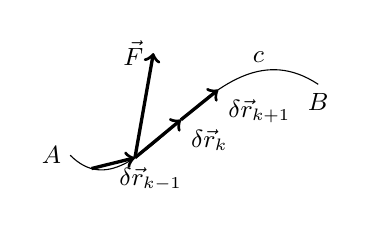
\begin{tikzpicture}[baseline={([yshift=-1em]current bounding box.north)},
scale=0.9]
\small
\clip(-0.6,-0.6) rectangle(3.9,1.8);
\draw (0,0) node[left] {$A$} .. controls (1,-1) and (2,2) .. (3.5,1)
            node[below] {$B$}
            node [pos=0.8,above] {$c$}
            coordinate [pos=0.1] (d)
            coordinate [pos=0.3] (a)
            coordinate [pos=0.5] (b)
            coordinate [pos=0.65] (c);
\draw [->,very thick] (d)--(a) node [below,xshift=2mm]{$\delta\vec r_{k-1}$};
\draw [->,very thick] (a)--(b) node [below right]{$\delta\vec r_k$};
\draw [->,very thick] (b)--(c) node [below right]{$\delta\vec r_{k+1}$};
\draw [very thick, ->] (a) --+(80:1.5) node[left]{$\vec F$};
\end{tikzpicture}\\
deslocamentos $\delta\vec r_k$, $k=1,2,\ldots N$. O
trabalho total realizado pela força $\vec F$ durante o deslocamento ao longo da
trajetória é igual à soma dos tralbalhos realizados em cada passo $\delta\vec
r_1$, $\delta \vec r_2$, \ldots Estes passos elementares são escolhidos
suficientemente pequenos para que se possam desprezar as variações de $\vec
F(\vec r)$ em cada um e portanto, nestas condições, o trabalho realizado em
cada porção do deslocamento pode ser calculado com a fórmula básica $\delta
W_k=\vec F\cdot\delta\vec r_k$.  Uma vez calculadas as contribuições dos
diferentes deslocamentos elementares, o trabalho total ao longo de todo o
deslocamento é obtido somando-os
\begin{equation*}
W\simeq \sum_{k=1}^N \delta W_k=
        \sum_{k=1}^N \vec F(\vec r_k)\cdot \delta \vec r_k.
\end{equation*}
Esta estimativa é apenas aproximada porque resulta de se desprezarem as
variações de $\vec F$ no interior de cada um dos pequenos deslocamentos $\delta
\vec r_k$. Podemos melhorar a aproximação reduzindo o tamanho desses pequenos
deslocamentos, e aumentando o seu número total $N$. Recuperamos o valor exato
tomando o limite de um número infinito deslocamentos infinitamente pequenos:
\begin{equation*}
W=\lim_{\substack{N\to\infty\\ \delta\vec r_k\to0}}\sum_{k=1}^N \vec F(\vec r_k)\cdot\delta\vec r_k.
\end{equation*}
O limite no lado direito desta igualdade chama-se \emph{integral de caminho} da
função vetorial $\vec F(\vec r)$ ao longo do caminho $c$ e representa-se como
\begin{equation}
\int_c\vec F(\vec r)\cdot d\vec r=\lim_{\substack{N\to\infty\\
\delta\vec r_k\to0}}\sum_{k=1}^N \vec F(\vec r_k)\cdot\delta\vec r_k.
\end{equation}
No contexto em que fizemos esta discussão, a função $\vec F$ é uma força e,
consequentemente, o integral de caminho é o trabalho que ela realiza. Mas a
noção de integral de caminho pode aplicar-se para qualquer função vetorial da
posição (velocidade do escoamento de um fluido, campo magnético, etc.).

A curva do espaço ao longo da qual se calcula o integral de caminho pode ser
fechada, ou seja, começar e acabar num mesmo ponto. Nesses casos, chamamos
\emph{circulação} ao integral de caminho. Para explicitar que um integral de
caminho é uma circulação, é costume decorar o símbolo de integral com um
círculo, como o que se apresenta no primeiro membro da equação seguinte (uma das
equações de Maxwell do eletromagnetismo):
\begin{equation*}
  \oint_c \vec E\cdot d\vec l = -\td{}{t}\int_{S}\vec B\cdot\hat ndS.
\end{equation*}

O sentido em que se faz o integral de caminho numa curva aberta é normalmente
fixado pelo que se considera início e fim da própria curva; mas, numa
circulação, o início e o fim coincidem, de forma que não se pode daí deduzir o
sentido da integração. Por isso, para concretizar o significado da circlação (e,
mais prosaicamente, o sinal do resultado) tem que se indicar em que sentido é
feito o cálculo.

Algumas funções vetoriais têm a particularidade de terem circulação nula,
qualquer que seja a curva de integração (desde que fechada, bem entendido).
Essas funções dizem-se \emph{conservativas}\footnote{Esta designação tem ainda
  que ver com as propriedades de alguns campos de forças: os casos em que as
  forças têm circulações necessariamente nulas são os casos em que se pode
aplicar o Princípio da Conservação da Energia Mecânica.}

\subsubsection*{Cálculo de integrais de caminho}
Em muitas situações importantes, o valor de um integral de caminho pode ser
deduzido sem serem necessários cálculos. Por exemplo, quando a função integranda
é uniforme, pode ser posta em evidência no integral, resultando então o simples
produto escalar com o deslocamento total. Ainda mais simples, se função
integranda for, em cada ponto, perpendicular à trajetória, o seu produto
escalar com o elemento de deslocamento é nulo; logo, é igualmente nulo o integral.

Mais em geral, o cálculo do integral de caminho
\begin{equation*}
I=\int_c\vec F(\vec r)\cdot d\vec r
\end{equation*}
passa por explicitar o produto escalar $\vec F(\vec r)\cdot d\vec r$ (usando a
fórmula geométrica $\vec F\cdot d\vec r=F dr\cos\theta$, ou a fórmula analítica
$\vec F\cdot d\vec r=F_xdx+F_ydy+F_zdz$) e por exprimir as variáveis envolvidas
na expressão resultante como funções de um parâmetro escalar que caracterize a
posição ao longo do caminho (por exemplo, a distância ao ponto inicial, medida
ao longo do caminho). Seguem-se alguns exemplos.

\begin{examples}
\item \label{ex:a} Calcule o valor do integral de caminho da função vetorial
uniforme $\vec A(\vec r)=\he_x/2+\he_y$ ao longo de uma semicircunferência no
plano $xy$, com raio $a$ e centro na origem, com início no ponto $A=(a,\,0)$ e
fim em $B=(-a,\,0)$.\\
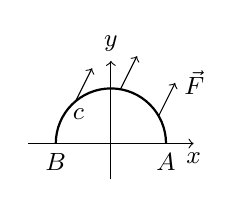
\begin{tikzpicture}[scale=0.7,baseline={([yshift=-10pt]current bounding
box.north)}]
\small
\draw [->](-1.5,0) -- (1.5,0) node [below] {$x$};
\draw [->] (0,-0.65) -- (0,1.5) node[above]{$y$};
\draw [thick](1,0) node[below]{$A$} arc (0:180:1) node[below]{$B$} node [pos=0.7,below]{$c$};
\draw [->] (30:1) --+(0.3,0.6) node [right]{$\vec F$};
\draw [->] (80:1) --+(0.3,0.6);
\draw [->] (130:1) --+(0.3,0.6);
\end{tikzpicture}\hfill
\begin{minipage}[t]{0.8\linewidth}
Como a função é uniforme, $\vec A$ pode ser posto em evidência no integral.
Então
\begin{align*}
\int_c\vec A(\vec r)\cdot d\vec r&=\vec A(\vec r)\cdot \int_c d\vec r=\vec
A\cdot\Delta\vec r= (\he_x/2+\he_y)\cdot(-2a\he_x) =-a.
\end{align*}
\end{minipage}

\item
    Repita o cálculo anterior, mas agora ao longo de outra porção da mesma
    circunferência, o arco compreendido entre $C=(0,-a)$ e $D=(0,a)$\\
    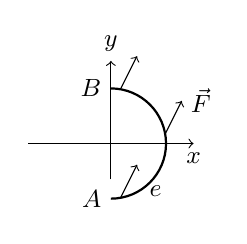
\begin{tikzpicture}[scale=0.7,
                        baseline={([yshift=-10pt]current bounding box.north)}]
    \small
    \draw [->](-1.5,0) -- (1.5,0) node [below] {$x$};
    \draw [->] (0,-0.65) -- (0,1.5) node[above]{$y$};
    \draw [thick](0,-1) node[left]{$A$} arc (-90:90:1) node[left]{$B$} node
    [pos=0.3,below]{$e$};
    \draw [->] (280:1) --+(0.3,0.6);
    \draw [->] (10:1) --+(0.3,0.6) node [right]{$\vec F$};
    \draw [->] (80:1) --+(0.3,0.6);
    \end{tikzpicture}\hfill
\begin{minipage}[t]{0.8\linewidth}
O cálculo é semelhante ao do exemplo anterior:
\begin{align*}
\int_e\vec A\cdot d\vec r&=\vec A\int_e d\vec r=(\he_x/2+\he_y)\cdot(-2a\he_y)
=-2a.
\end{align*}
\end{minipage}
\item
    Mostre que as funções uniformes são conservativas.
\item Calcule o integral de caminho da função $\vec A=\vec r/2$ ao longo do caminho do
Exemplo~\ref{ex:a}\\
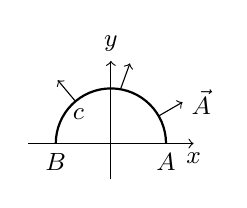
\begin{tikzpicture}[scale=0.7,baseline={([yshift=-10pt]current bounding
box.north)}]
\small
\draw [->](-1.5,0) -- (1.5,0) node [below] {$x$};
\draw [->] (0,-0.65) -- (0,1.5) node[above]{$y$};
\draw [thick](1,0) node[below]{$A$} arc (0:180:1) node[below]{$B$} node [pos=0.7,below]{$c$};
\draw [->] (30:1) --+(30:0.5) node [right]{$\vec A$};
\draw [->] (80:1) --+(70:0.5);
\draw [->] (130:1) --+(130:0.5);
\end{tikzpicture}\hfill
\begin{minipage}[t]{0.8\linewidth}
A função integranda é, em cada ponto, perpendicular ao caminho de integração.
Logo, $\vec A\cdot d\vec r=0$, e o integral anula-se também.
\end{minipage}
\item
Agora, um exemplo menos trivial: calcule o integral de caminho da função $\vec
A=\vec r/2$ do exemplo anterior, ao longo do segmento de reta que une os pontos
$(0,\,a)$ e $(b,\,0)$, com $a,\,b>0$.\\
\begin{tikzpicture}[scale=0.7,
                    baseline={([yshift=-10pt]current bounding box.north)}]
\small
\coordinate(O) at (0,0);
\draw [->](-.25,0) -- (2.0,0) node [right] {$x$};
\draw [->] (0,-0.25) -- (0,1.25) node[left]{$y$};
\coordinate (A) at (0,0.75);
\coordinate (B) at (1.5,0);
\draw [thick] (0,0.75) node [left]{$a$} -- (1.5,0) node [below]{$b$}
    coordinate [pos=0.2] (a)
    coordinate [pos=0.5] (b)
    coordinate [pos=0.8] (c);
\draw [->] (a) -- ($ (a)!-0.5!(O) $);
\draw [->] (b) -- ($ (b)!-0.5!(O) $) node [above] {$\vec A$};
\draw [->] (c) -- ($ (c)!-0.5!(O) $);
\draw ($ (B)!7mm!(A) $) arc (180-atan(0.5):180:7mm)
node [shift={(-4pt,4pt)}] {$\alpha$};
\end{tikzpicture}\hfill
\begin{minipage}[t]{0.8\linewidth}
Seja $\alpha=\arctan(a/b)$ o ângulo entre a direção do caminho de integração e o
eixo dos $x$. Então, em todos os pontos do caminho de integração, temos
\begin{align*}
y&=a-x\tan\alpha & dy&=-\tan\alpha\,dx & d\vec r&=(dx,\,dy)\\
\vec A&=\frac{\vec r}{2}= \left(\frac{x}{2},\,\frac{y}{2}\right)
\end{align*}
\end{minipage}
Assim sendo, podemos escrever
\begin{align*}
\vec A\cdot d\vec r&=\frac{x}{2}dx+\frac{y}{2}dy=\frac{x}{2}dx+
\frac{a-\tan\alpha\,x}{2}(-\tan\alpha\,dx)\\
&=\frac{x}{2}\left(1+\tan^2\alpha\right)dx-\frac{a}{2}\tan\alpha\,dx
\end{align*}
E, por fim,
\begin{equation*}
\int_c\vec A\cdot d\vec r=\int_0^b\left[
\frac{x}{2}\left(1+\tan^2\alpha\right)-\frac{a}{2}\tan\alpha\right]\,dx=
\frac{b^2}{4}\left(1+\tan^2\alpha\right)-\frac{ab}{2}\tan\alpha
=\frac{b^2-a^2}{4}
\end{equation*}
Note-se que se escreveu o produto escalar como a soma dos produtos das
componentes homónimas dos dois vetores $\vec A$ e $d\vec r$ (fórmula analítica)
e se usou a variável $x$ como parâmetro de posição ao longo do caminho de
integração.
\end{examples}

\subsection{Fluxo}
Dada uma função vetorial uniforme $\vec A$ e uma superfície plana com área
$\Delta S$ e versor normal $\hat n$, chama-se \emph{fluxo}\footnote{A designação
\emph{fluxo} vem da mecância de fluidos. No escoamento de um fluido, o
\emph{fluxo} (no sentido agora definido) da função velocidade do fluido através
de uma dada superfície é igual ao \emph{fluxo} que a atravessa (no sentido de
volume de fluido que passa através da superfície por unidade de tempo).}
de $\vec A$ através da superfície no sentido de $\hat n$ ao produto escalar
\begin{equation*}
\Delta \Phi=\vec A\cdot \hat n\,\Delta S.
\end{equation*}
Intuitivamente, esta variável dá expressão quantitativa à noção vaga da
``quantidade de função'' que atravessa a superfície. Com essa noção vaga,
esperamos que o fluxo seja maior quando a função é mais intensa, ou quando a
área da superfície considerada aumenta, e ainda quando a função é perpendicular
à superfície que, assim, consegue ``apanhar'' mais campo.\footnote{Só um
exemplo: colocamos um tubo de ensaio debaixo de um chuveiro; enchemo-lo mais
rapidamente se o caudal do chuveiro for intenso (módulo de $\vec A$ elevado), ou
se a boca do tubo for larga (grande área $S$) ou se virarmos a boca do tubo bem
na direção dos jatos de água do chuveiro (superfície perpendicular à função).}

Nos casos em que a função não é uniforme e/ou a superfície não é plana,
aplica-se um procedimento semelhante ao usado para os integrais de caminho:
divide-se a superfície de integração num grande número de elementos muito
pequenos, tão pequenos que as variações da função e a curvatura da superfície se
podem desprezar dentro de cada um. Nesta aproximação (que é exata no limite em
que o número de elementos de área tende para infinito e eles se tornam
infinitesimais) podemos aplicar a expressão acima apresentada para calcular o
fluxo da função através de cada elemento, e somar os vários resultados para
obter o fluxo total através da superfície. O fluxo de uma função genérica $\vec
A$ (não necessariamente uniforme) através de uma superfície $S$ (não
necessariamente plana) fica assim definido como
\begin{equation*}
\Phi = \int_S \vec A\cdot\hat n \, dS =
\lim_{\substack{N\to\infty\\\delta S_k\to0}}
\sum_{k=1}^N\vec A\cdot\hat n_k\,\delta S_k,
\end{equation*}
onde $\hat n$ representa o versor normal à superfície em cada ponto e $\hat n_k$
o versor normal a cada elemento de área considerado.

\subsubsection*{Cálculo do fluxo}
Há muitas situações (principalmente em aplicações pedagógicas) em que o cálculo
do fluxo é particularmente simples. Por exemplo, se a função $\vec A$ for, em
todos os pontos, tangente à superfície atrvés da qual se calcula o fluxo, o
resultado é obviamente nulo, uma vez que, sendo tangente à superfície, a função
$\vec A$ é perpendicular à normal $\hat n$; logo, a função integranda é nula e
portanto é nulo o integral.

Por outro lado, quando a função é perpendicular à superfície em todos os pontos,
ela tem a direção da normal. O produto escalar fica então, à parte um sinal
dependente dos sentidos de $\vec A$ e $\hat n$ igual ao produto das
normas dos dois vetores envolvidos (e a de $\hat n$ é, por definição, igual a
1). Nestes casos a fórmula do fluxo reduz-se pois a 
\begin{equation*}
\Phi = \int_S A\,dS,\qquad\text{ se $\vec A$ é perpendicular a $S$.}
\end{equation*}

Outro caso que permite uma grande simplificação é o das funções uniformes.
Note-se que mesmo sendo $\vec A$ uniforme, a função integranda não é constante
porque o produto escalar $\vec A\cdot \hat n$ depende de ponto para ponto quando
a superfície não é plana. Ainda assim, temos:
\begin{equation*}
\Phi=\int_S\vec A\cdot\hat n\,dS=\int_S A\cos\theta\,dS=A\int_s\cos\theta\,dS,
\end{equation*}
onde $\theta$ é o ângulo entre $\vec A$ e $\hat n$. Mas $dS \cos\theta$ é (à
parte um sinal eventual dependendo da orientação de $\vec A$ e de $\hat n$) a área
da projeção do elemento infinitesimal de superfície $dS$ no plano perpendicular
a $\vec A$. Então, concluímos que o fluxo de uma função uniforme através de uma
dada superfície é igual ao módulo dessa fução multiplicado pelo valor da área da
projeção da superfície no plano perpendicular à função:
\begin{equation*}
\int_S\vec A\cdot\hat n\,dS= AS_{\text{prj}},\qquad\text{ se $\vec A$ for
uniforme.}
\end{equation*}

Mais em geral, e como para os integrais de caminho, é necessário explicitar o
produto escalar no integrando e exprimir todas as vriáveis como função de duas 
coordenadas que identifiquem a posição na superfície de integração, após o que
se realiza a integração (dupla) propriamente dita. Analizam-se a seguir alguns
exemplos.

\begin{examples}
\item Fluxo de $\vec r$ através da superfície de um quadrado de lado $a$ situado
no plano $xy$, com centro na origem, com os lados paralelos aos eixos
coordenados.\\
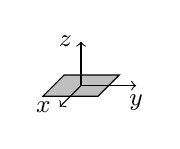
\begin{tikzpicture}[scale=0.7,
                    baseline={([yshift=-10pt]current bounding box.north)}]
\small
\draw [fill=gray!50] (-0.5,0,-0.5) -- (0.5,0,-0.5) -- (0.5,0,0.5) --(-0.5,0,0.5) -- cycle; 
\draw [->] (0,0,0) -- (0,0,1) node [left]{$x$};
\draw [->] (0,0,0) -- (0,0.8,0) node [left]{$z$};
\draw [->] (0,0,0) -- (1,0,0) node [below]{$y$};
\end{tikzpicture}\hfill
\begin{minipage}[t]{0.85\linewidth}
Em coordenadas cartesianas a função dada é 
$\vec r=x\he_x+y\he_y+z\he_z\equiv(x,\,y,\,z)$; mas, nos pontos da superfície
considerada (situada no plano $xy$) $z=0$, de modo que, para os efeitos pretendidos, podemos
escrever $\vec r=(x,\,y,\,0)$, isto é, por outras palavras, a função\linebreak 
\vspace{-0.7\baselineskip}
\end{minipage}
dada é tangente à superfície de integração. Assim sendo, o produto escalar
envolvido no cálculo do fluxo é nulo; logo, o integral anula-se também.
\item
    Fluxo de uma função radial $\vec F(\vec r)=F(r)\hat u_r$ através de uma
    superfície esférica com centro na origem.\\
    \tdplotsetmaincoords{60}{120}
    \begin{tikzpicture}[tdplot_main_coords,
                    baseline={([yshift=-10pt]current bounding box.north)}]
        \small
        \pgfmathsetmacro\R{0.7}
        \coordinate(O) at (0,0,0);
        \fill [tdplot_screen_coords,ball color=gray!05] circle(\R);

        \pgfmathsetmacro\theta{45}
        \pgfmathsetmacro\phi{70}
        \pgfmathsetmacro\dtheta{20}
        \pgfmathsetmacro\dphi{20}
        \tdplotsetcoord{P}{\R}{\theta}{\phi}
        \node at(P) [shift={(-0.7mm,1.4mm)}] {$ds$};
        \tdplotsetcoord{C}{\R}{\theta+0.5*\dtheta}{\phi+0.5*\dphi}
        \draw [thick,->] (C) -- ($ (C)!-0.45cm!(O) $) node[below] {$\hat n$};
        \draw [->] (C) -- ($ (C)!-0.7cm!(O) $) node[below right] {$\vec F$};
        \tdplotdrawarc[ultra thin]
                        {(0,0,{\R*cos(\theta)})}{{\R*sin(\theta)}}%
                        {\phi}{\phi+\dphi}{}{}
        \tdplotdrawarc[ultra thin]
                        {(0,0,{\R*cos(\theta+\dtheta)})}{{\R*sin(\theta+\dtheta)}}%
                        {\phi}{\phi+\dphi}{}{}
        \tdplotsetthetaplanecoords{\phi}
        \tdplotdrawarc[tdplot_rotated_coords,ultra thin]
                        {(O)}{\R}{\theta}{\theta+\dtheta}{}{}
        \tdplotsetthetaplanecoords{\phi+\dphi}
        \tdplotdrawarc[tdplot_rotated_coords,ultra thin]
                        {(O)}{\R}{\theta}{\theta+\dtheta}{}{}
    \end{tikzpicture}\hfill
    \begin{minipage}[t]{0.83\linewidth}
    Como a função é radial (dirigida para o centro), é perpendicular à
    superfície de integração; assim, $\vec F(\vec r)\cdot\hat n=\pm F(r)$ (o
    sinal é positivo se o sentido da função for para fora, e negativo se for
    para dentro. Por outro lado, todos os pontos da superfície estão à mesma
    distância $r$ do centro; ou seja, o módulo da função $\vec F$ é constante
    neste\linebreak\vspace{-0.7\baselineskip}
    \end{minipage}
    integral e pode por isso ser posto em em evidência. Juntando tudo, temos:
    \begin{equation*}
    \int_S\vec F(\vec r)\cdot\hat n\,dS=\int_SF(r)dS=F(r)\int_SdS=4\pi r^2F(r).
    \end{equation*}
    \item
        Cálculo do fluxo da função $\vec F(\vec r)=h\he_z$ ($h$ constante)
        através da calote semisférica com centro na origem, raio $a$, situada no
        lado $z>0$.\\
        \pgfmathsetmacro{\elv}{60}
        \pgfmathsetmacro{\azi}{120}
        \tdplotsetmaincoords{\elv}{\azi}
        \begin{tikzpicture}[scale=0.75,tdplot_main_coords,
                            baseline={([yshift=-10pt]current bounding box.north)}]
            \small
            \pgfmathsetmacro{\R}{2}
            \draw[thin,->] (0,0,0) -- (1.2*\R,0,0) node[anchor=north east]{$x$};
            \draw[thin,->] (0,0,0) -- (0,1.2*\R,0) node[anchor=north west]{$y$};
            \draw[thin,->] (0,0,0) -- (0,0,1.25*\R) node[anchor=south]{$z$};

            \draw ({\R*cos(\azi/2)},{\R*sin(-\azi/2)},0) arc ({-\azi/2}:\azi:\R);
            \draw (-\R*1cm,0) arc(180:0:\R*1cm);
            \pgfmathsetmacro{\auxv}{\R*cos(\elv)}
            \shade[ball color=blue!10!white,opacity=0.2] (\R*1cm,0)
                arc (0:-180:\R*1cm and \auxv*1cm) arc (180:0:\R*1cm and \R*1cm);

            \pgfmathsetmacro{\T}{30}
            \pgfmathsetmacro{\P}{50}
            \pgfmathsetmacro{\dT}{12}
            \pgfmathsetmacro{\dP}{15}
            \tdplotsetcoord{A}{\R}{\T}{\P}
            \tdplotsetcoord{B}{\R}{\T+\dT}{\P}
            \tdplotsetcoord{C}{\R}{\T+\dT}{\P+\dP}
            \tdplotsetcoord{D}{\R}{\T}{\P+\dP}

            \draw [thin,densely dashed] (A)--(Axy);
            \draw [thin,dashed] (B)--(Bxy);
            \draw [thin,dashed] (C)--(Cxy);
            \draw [thin,dashed] (D)--(Dxy);
            \draw [fill=gray!50](Axy)--(Bxy)--(Cxy)--(Dxy) -- cycle;
            \node at (Bxy) [shift={(0.3,-0.1)}]{$dS\cos\theta$};

            \tdplotdrawarc{((0,0,{\R*cos(\T)})}{{\R*sin(\T)}}{\P}{\P+\dP}{}{}
            \tdplotdrawarc{((0,0,{\R*cos(\T+\dT)})}{{\R*sin(\T+\dT)}}%
                {\P}{\P+\dP}{}{}
            \tdplotsetthetaplanecoords{\P}
            \tdplotdrawarc[tdplot_rotated_coords] {(0,0,0)}{\R}{\T}{\T+\dT}{}{}
            \tdplotsetthetaplanecoords{\P+\dP}
            \tdplotdrawarc[tdplot_rotated_coords]
                            {(0,0,0)}{\R}{\T}{\T+\dT}{right}{$dS$}
            \coordinate(O) at (0,0,0);
            \tdplotsetcoord{P}{\R}{\T+0.5*\dT}{\P+0.5*\dP}
            \draw [->] (P) -- ($ (P)!-8mm!(O) $) node[below right] {$\hat n$};
            \draw [thick,->] (P) -- +(0,13mm) node[below right]{$\vec F$};

            \tdplotsetthetaplanecoords{\P+0.5*\dP}
            \tdplotdrawarc[tdplot_rotated_coords,ultra thin]
                            {(P)}{0.9}{0}{\T+0.5*\dT}{shift={(0.2,0.2)}}{$\theta$}

            \tdplotsetthetaplanecoords{0}
            \tdplotdrawarc[ultra thin,tdplot_rotated_coords]{(0,0,0)}{\R}{-5}{5}{}{}
            \tdplotsetthetaplanecoords{90}
            \tdplotdrawarc[ultra thin,tdplot_rotated_coords]{(0,0,0)}{\R}{-5}{5}{}{}
        \end{tikzpicture}
        \hfill
        \begin{minipage}[t]{0.72\linewidth}
        Como a função dada $\vec F$ é uniforme (tem os mesmos módulo e
        orientação em todos os pontos), a expressão do fluxo pode ser
        simplificada:
        \begin{equation*}
        \Phi=\int_S\vec F\dot\hat n\,dS=\int_S h\cos\theta\,dS=h\int_S\cos\theta\,dS.
        \end{equation*}
        Mas $ds\cos\theta$ é a área da projeção do elemento de superfície $dS$
        no plano $xy$ (o plano perpendicular a $\vec F$. Então o integral em
        cima é simplesmente igual à área da projeção da calote semiesférica no
        plano $xy$, ou seja, $\pi a^2$. Então,
        \begin{equation*}
        \Phi=\int_S\vec F\cdot\hat n\,dS=\pi a^2 h.
        \end{equation*}
        \end{minipage}
\end{examples}

\subsection{Integrais e testes de avaliação}
O cálculo de integrais múltiplos pode ser bastante complicado. Mas nos testes
não serão nunca exigidos integrais difíceis. Mas é importante ter uma ideia
nítida do que é um integral, o que representam intuitivamente de um ponto de
vista matemático. Sabido isso, será sempre trivial determinar o valor dos
integrais com que se confrontarem nos testes. Dito isto, devo ainda acrescentar
que a melhor maneira de adquirir esta intuição é calcular integrais. Muitos. Dos
simples e também dos complicados.

\section{Operadores diferenciais}
As equações de Maxwell são quatro equações às derivadas parciais dos campos
elétrico e magnético que traduzem localmente\footnote{Isto é, como igualdades
que relacionam o valor de funções em cada ponto do espaço.} as leis integrais
do eletromagnetismo que foram estudadas na cadeira de Física Geral II, a saber:
a lei de Gauss do campo elétrico (e uma que desempenha um papel semelhante para
o campo magnético), a lei de Faraday e a lei de Ampère. Estas equações envolvem
os operadores diferenciais divergência e rotacional, que vamos agora,
rapidamente, recordar.

\subsection*{Divergência de um campo vetorial}
A divergência de um campo vetorial é um escalar igual ao fluxo do campo atrvés
de uma superfície fechada por unidade de volume.  De um modo talvez mais
intuitivo (mas muito menos preciso), podemos dizer que é a \emph{``quantidade''
de campo que ``sai''} desse ponto por unidade de volume. A
Figura~\ref{fig:10-020} ilustra este significado intuitivo da divergência de um
campo vetorial.
\begin{figure}[htb]
  {\centering
    \begin{tikzpicture}
	\small
	\coordinate(P) at (-2,0);
	\coordinate(Q) at (2,0);
	\foreach \q in {0,30, 60, 90, 120,150,180,210,240,270,300,330} {
		\draw [->-] (P) -- +(\q:1cm);
		\draw [-<-] (Q) -- +(\q:1cm);
	};
	\node at (P) [shift={(3mm,-3mm)}, fill=white,inner sep=2pt]{$P$};
	\node at (Q) [shift={(3mm,-3mm)}, fill=white,inner sep=2pt]{$Q$};
\end{tikzpicture}
\par
  }
  \caption{À esquerda, exemplo de um campo com divergência positiva no ponto
  $P$; à direita o campo tem divergência negativa no ponto
  $Q$.\label{fig:10-020}}
\end{figure}


Pode demonstrar-se (mas não o faremos aqui) que, usando coordenadas cartesianas,
a divergência de um campo vetorial $\vec V$ é dada por
\begin{equation}\label{eq:divcart}
  \div\vec V=\pd{V_x}{x} + \pd{V_y}{y}+\pd{V_z}{z}.
\end{equation}
Esta expressão é formalmente semelhante ao produto escalar do operador vetorial
$\vec\nabla$ da eq.~\eqref{eq:cartnabla} com $\vec V$, e por isso pode també
escrever-se
\begin{equation}
  \div\vec V=\vec\nabla\cdot\vec V.
\end{equation}
o produto escalar de nabla e $\vec V$:

Em coodenadas polares cilíndricas $(\rho,\,\varphi,\,z)$, a divergência de um campo
vetorial $\vec V=V_r\he_r+V_\varphi\he_\varphi+V_z\he_z$ tem a forma
\begin{equation}
\div\vec V=\frac{1}{\rho}\pd{(\rho V_\rho)}{\rho}
    +\pd{V_\varphi}{\varphi}+\pd{V_z}{z}
\end{equation}
e, em coordenadas polares esféricas $(r,\,\theta,\,\varphi)$, 
\begin{equation}
\div \vec V=\frac{1}{r^2}\pd{(r^2V_r)}{r}+
    \frac{1}{r\sin\theta}\pd{}{\theta}(V_\theta\sin\theta)+
    \frac{1}{r\sin\theta}\pd{V_\varphi}{\theta}
\end{equation}

\subsection*{Rotacional de um campo vetorial}
O rotacional de um campo vetorial é um vetor igual à circulação do campo por
unidade de área. A sua direção é a perpendicular ao plano onde a circulação tem
o valor máximo. Em termos intuitivos (mas terivelmente imprecisos), o rotacional
dá uma ideia de \emph{``quanto'' é que o campo ``roda''} num ponto; a sua
direção é do ``eixo'' dessa ``rotação'' e o sentido é o dado pela regra da mão
direita a partir do sentido da ``rotação'' do campo. 

O rotacional de um campo $\vec V$ é, em coordenadas cartesianas, dado por
\begin{equation}\label{eq:rotcart}
  \rot\vec V=
  \left(\pd{V_z}{y}-\pd{V_y}{z},\; \pd{V_x}{z}-\pd{V_z}{x},\;
  \pd{V_y}{x}-\pd{V_x}{y}\right).
\end{equation}
Em termos do símbolo vetorial nabla, fica, mais sucintamente,
\begin{equation}
  \rot\vec V=\vec\nabla\times\vec V.
\end{equation}

Usando a primeira das igualdades da eq.~\eqref{eq:tcp}, encontramos uma
expressão para o rotacional do rotacional de um campo vetorial, que será útil
quando estuidarmos as ondas eletromagnéticas:
\begin{align}
\rot\rot \vec V&=\vec\nabla\times\vec\nabla\times\vec V=
\vec \nabla(\vec\nabla\cdot\vec V)-\nabla^2\vec V\nonumber\\
&=\grad\div \vec V-\lap\vec V,
\end{align}
onde $\lap\vec A$ representa o \emph{laplaciano} do campo vetorial $\vec V$, um
operador diferencial de segunda ordem, igual à soma das duplas derivadas não
cruzadas do campo,
\begin{equation}
\lap F =
\pdd{F}{x}+
\pdd{F}{y}+
\pdd{F}{z},\qquad\text{para qualquer função escalar ou vetorial $F$}
\end{equation}
{\small%
  Feita esta abreviadíssima explicação sobre os operadores $\div$ e $\rot$,
  talvez não seja pior referir alguns factos mais básicos da ``vida secreta
  das derivadas''. Uma função crescente tem uma variação positiva quando a
  variável de que depende sofre um acréscimo; logo, a sua taxa de variação
  (variação da função a dividir pelo acréscimo da variável) é positiva, logo a
  sua derivada (outro nome para a taxa de variação) é positiva. Do mesmo modo,
  uma função decrescente tem derivada negativa. Uma função constante não é
  crescente nem decrescente; logo, não tem derivada positiva nem negativa, tem
  derivada nula.  Uma função que atinge um valor extremo (máximo ou mínimo) para
  um dado valor da variável de que depende, nesse ponto não é crescente nem
  decrescente: tem derivada nula nesse ponto.

  Quando estudamos funções de várias variáveis (como é o caso agora), estas
  regras ainda se aplicam mas têm que ser consideradas com cuidado porque a
  função pode ser crescente relativamente aos acréscimos de uma variável,
  decrescente com acréscimos de outra variável e constante com acréscimos de uma
  terceira variável. Assim, uma função que depende da posição e do tempo e que
  num dado ponto tem um valor que vai paulatinamente aumentando à medida que o
  tempo passa, é uma função que tem, nesse ponto, derivada temporal positiva. Se
  o seu valor num dado ponto se mantém inalterado com a passagem do tempo, então
  a sua derivada temporal, nesse ponto, é nula. E etc, etc, etc, acho que destes
  dois exemplos já se vai percebendo a lógica geral.

  A derivada de uma função de várias variáveis em ordem a uma delas é ainda, em
  geral, uma função dessas mesmas variáveis. Como tal, pode fazer sentido
  derivá-la novamente, em ordem à mesma variável ou em ordem a outra qualquer. O
  teorema de Swartz garante que esta derivada não depende da ordem com que se
  fazem cada uma das derivações:
  \begin{equation*}
    \cpdd{f}{x}{y}=
    \cpdd{f}{y}{x},\qquad\text{qualquer que seja a função $f$}
  \end{equation*}
}

